\documentclass[xcolor=table]{beamer}

% \rowcolors{1}{gray!30}{gray!10}

\usetheme{Boadilla}
\usecolortheme{dolphin}
\useoutertheme[subsection=false]{smoothbars}

\setbeamercolor{frametitle}{fg = black, bg = white} 
\setbeamercolor{palette primary}{use=structure,fg=white,bg=structure.fg!60!white}
\setbeamercolor{palette secondary}{use=structure,fg=white,bg=structure.fg!90!white}
\setbeamercolor{palette tertiary}{use=structure,fg=white,bg=structure.fg!120!white}
\setbeamercolor{palette quaternary}{use=structure,fg=black,bg=white} %Top bar

\setbeamertemplate{enumerate subitem}[circle]%
\renewcommand{\insertsubenumlabel}{\alph{enumii}}

\usepackage{amsmath}
\usepackage{xcolor}
\usepackage{booktabs}
\usepackage[utf8]{inputenc}
\usepackage{hyperref}
\usepackage[table]{xcolor}
\usepackage{setspace}
\usepackage{parskip}

\definecolor{lightgray}{gray}{0.9}

\hypersetup{
    colorlinks,
    citecolor=blue,
    linkcolor=blue
}

\usepackage{listings} %include R code

\definecolor{codegreen}{rgb}{0,0.6,0}
\definecolor{codegray}{rgb}{0.5,0.5,0.5}
\definecolor{codepurple}{rgb}{0.58,0,0.82}
\definecolor{backcolour}{rgb}{0.95,0.95,0.92}

\lstdefinestyle{mystyle}{
    backgroundcolor=\color{backcolour},   
    commentstyle=\color{codegreen},
    keywordstyle=\color{magenta},
    numberstyle=\tiny\color{codegray},
    stringstyle=\color{codepurple},
    basicstyle=\ttfamily\tiny,
    breakatwhitespace=false,         
    breaklines=true,                 
    captionpos=b,                    
    keepspaces=true,                 
    numbers=left,                    
    numbersep=5pt,                  
    showspaces=false,                
    showstringspaces=false,
    showtabs=false,                 
    columns=fullflexible,
    frame=single,
    tabsize=2
}

\lstset{style=mystyle}


\author{Jonathan P. Latner, PhD}
\title{Balancing efficiency, utility, and privacy}
\date{\today}

\beamertemplatenavigationsymbolsempty 
\setbeamerfont{page number in head/foot}{size=\tiny}
\setbeamertemplate{footline}[frame number]
\setbeamertemplate{caption}[numbered]
\setbeamertemplate{section in toc}[sections numbered]

\begin{document}

\section{sd2011}
\begin{frame}[fragile]{Data - SD2011}

\begin{lstlisting}[firstnumber=1, label=glabels, xleftmargin=10pt,frame=single] 
'data.frame':   5000 obs. of  35 variables:
 $ sex       : Factor w/ 2 levels "MALE","FEMALE": 2 1 2 2 2 1 2 1 2 2 ...
 $ age       : num  57 20 18 78 54 20 39 39 43 63 ...
 $ agegr     : Factor w/ 6 levels "16-24","25-34",..: 4 1 1 6 4 1 3 3 3 5 ...
 $ placesize : Factor w/ 6 levels "URBAN 500,000 AND OVER",..: 3 6 1 6 3 3 6 3 6 5 ...
 $ region    : Factor w/ 16 levels "Dolnoslaskie",..: 5 10 7 10 16 12 15 5 13 1 ...
 $ edu       : Factor w/ 4 levels "PRIMARY/NO EDUCATION",..: 2 2 2 1 2 3 3 3 3 3 ...
 $ eduspec   : Factor w/ 27 levels "agriculture, forestry, fishing",..: 19 25 25 25 1 25 4 22 20 25 ...
 $ socprof   : Factor w/ 9 levels "EMPLOYED IN PRIVATE SECTOR",..: 6 7 7 6 3 7 2 1 2 6 ...

...

 $ nofriend  : num  6 4 20 0 6 10 0 4 1 25 ...
 $ smoke     : Factor w/ 2 levels "YES","NO": 2 2 2 2 1 2 2 2 1 1 ...
 $ nociga    : num  NA NA NA NA 20 NA NA NA 30 15 ...
 $ alcabuse  : Factor w/ 2 levels "YES","NO": 2 2 2 2 2 2 2 2 2 2 ...
 $ alcsol    : Factor w/ 2 levels "YES","NO": 2 2 2 2 2 2 2 2 2 2 ...
 $ workab    : Factor w/ 2 levels "YES","NO": 2 2 NA 2 2 2 2 2 2 2 ...
 $ wkabdur   : Factor w/ 32 levels "0","1","10","11",..: NA NA NA NA NA NA NA NA NA NA ...
 $ wkabint   : Factor w/ 3 levels "YES, TO EU COUNTRY",..: 3 3 3 3 3 3 3 3 3 3 ...
 $ wkabintdur: Factor w/ 5 levels "LESS THAN 1 YEAR",..: NA NA NA NA NA NA NA NA NA NA ...
 $ emcc      : Factor w/ 17 levels "AUSTRIA","BELGIUM",..: NA NA NA NA NA NA NA NA NA NA ...
 $ englang   : Factor w/ 3 levels "ACTIVE","PASSIVE",..: 3 1 1 3 3 1 2 3 3 3 ...
 $ height    : num  170 187 165 160 158 165 168 171 167 155 ...
 $ weight    : num  89 82 50 78 50 65 68 86 54 65 ...
 $ bmi       : num  30.8 23.4 18.4 30.5 20 ...
\end{lstlisting}

\end{frame}

\frame{\frametitle{Efficiency}
\begin{figure}
    \caption{}
    \resizebox{\textwidth}{!}{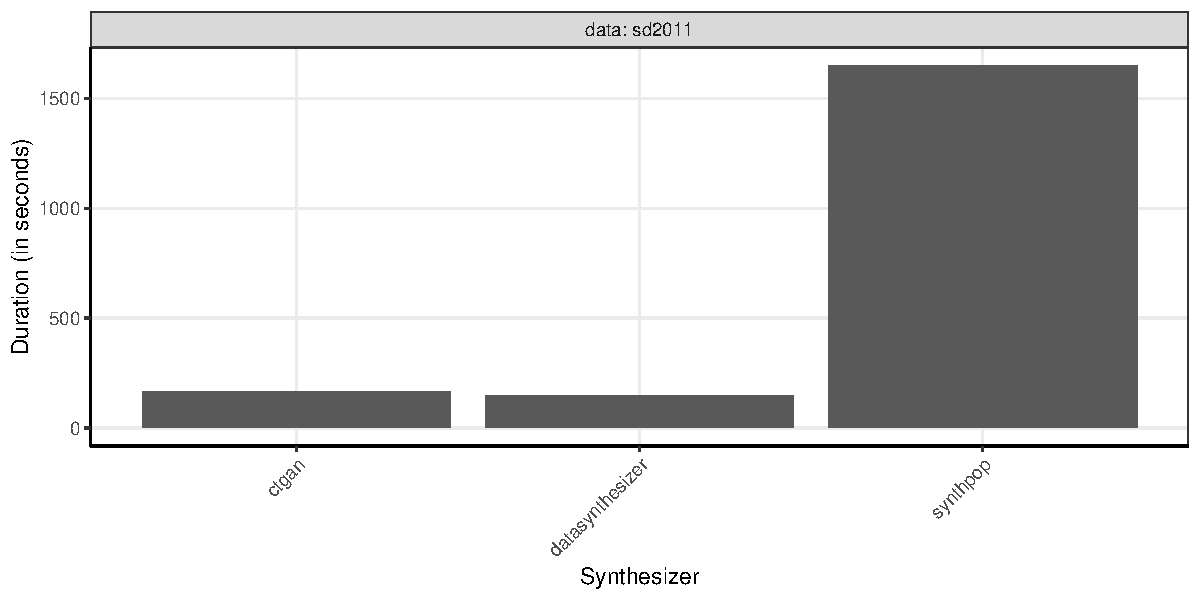
\includegraphics{../data/benchmark/graphs/graph_compare_duration.pdf}}
    \label{}
\end{figure}
}

\frame{\frametitle{Synthpop utility - two-way utility}
\begin{figure}
    \caption{}
    \resizebox{\textwidth}{!}{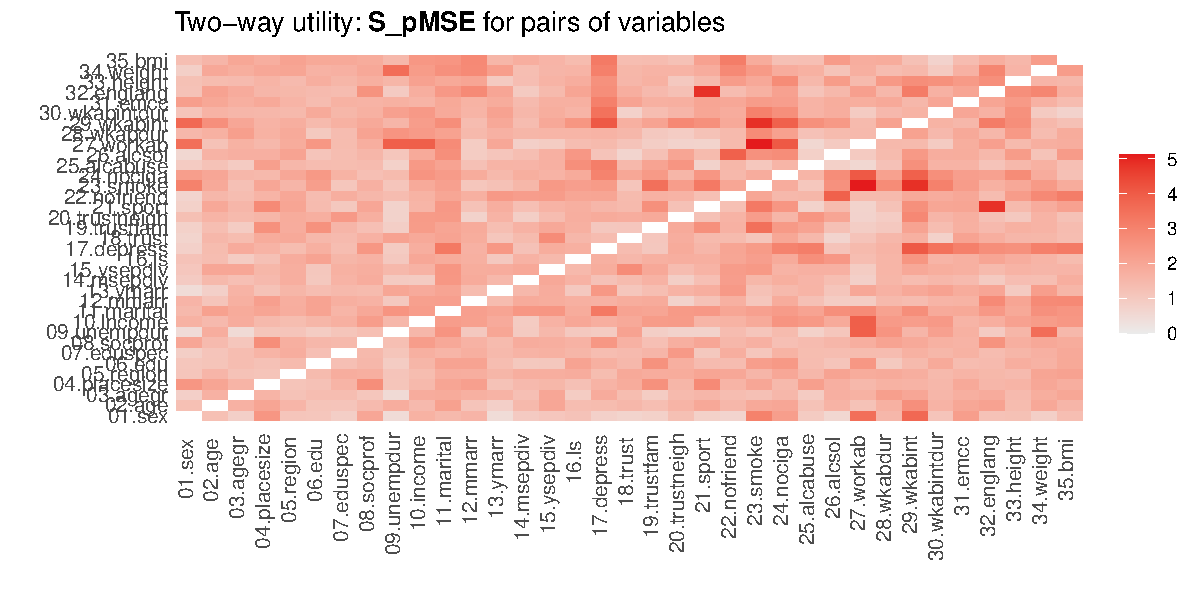
\includegraphics{../data/benchmark/graphs/synthpop/graph_synthpop_sd2011_two-way_utility.pdf}}
    \label{}
\end{figure}
}

\frame{\frametitle{DataSynthesizer utility - two-way utility}
\begin{figure}
    \caption{}
    \resizebox{\textwidth}{!}{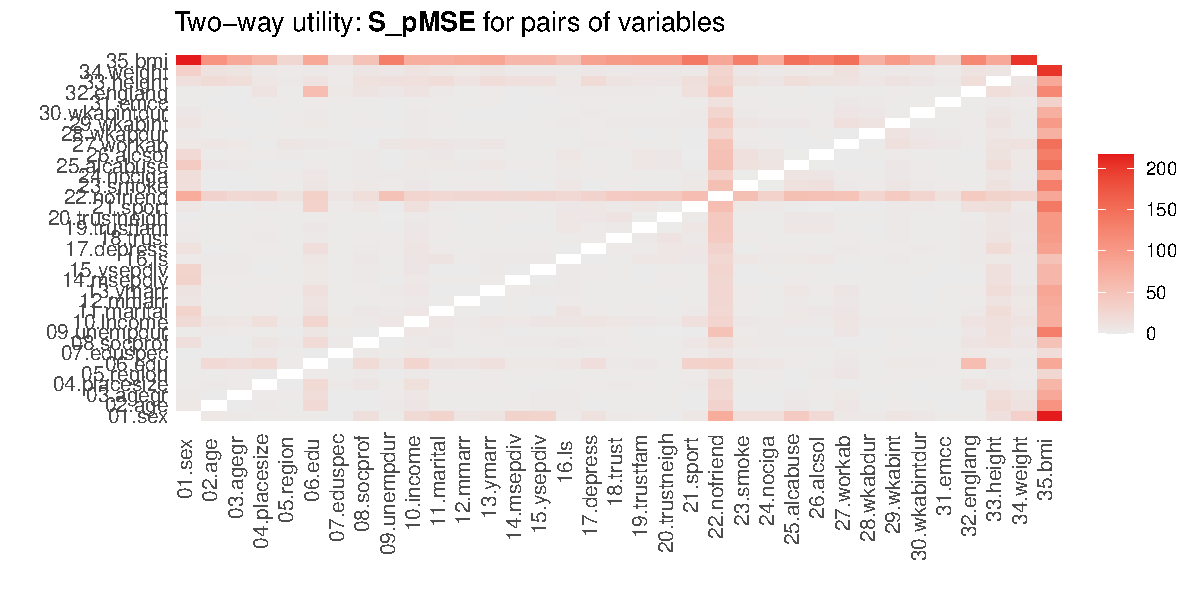
\includegraphics{../data/benchmark/graphs/datasynthesizer/graph_datasynthesizer_sd2011_two-way_utility.pdf}}
    \label{}
\end{figure}
}

\begin{frame}[fragile]{Kolmogorov-Smirnov statistic for full data set}

DataSynthesizer
\begin{lstlisting}[firstnumber=1, label=glabels, xleftmargin=10pt,frame=single] 
> utility_measure <- utility.gen(sds_list, df_ods, print.stats = "all", nperms = 3)
> utility_measure$SPECKS
     D 
0.6964 
\end{lstlisting}
Synthpop
\begin{lstlisting}[firstnumber=1, label=glabels, xleftmargin=10pt,frame=single] 
> utility_measure$SPECKS
     D 
0.2346
\end{lstlisting}

\end{frame}

\begin{frame}[fragile]{Kolmogorov-Smirnov statistic for each variable}

DataSynthesizer
\begin{lstlisting}[firstnumber=1, label=glabels, xleftmargin=10pt,frame=single] 
> df_compare$tab.utility[,4]
       sex        age      agegr  placesize     region        edu    eduspec    socprof 
    0.0064     0.0114     0.0084     0.0104     0.0200     0.0066     0.0158     0.0130 
  unempdur     income    marital      mmarr      ymarr    msepdiv    ysepdiv         ls 
    0.0038     0.0340     0.0070     0.0092     0.0160     0.0048     0.0044     0.0124 
   depress      trust   trustfam trustneigh      sport   nofriend      smoke     nociga 
    0.0102     0.0114     0.0014     0.0074     0.0022     0.1762     0.0010     0.0048 
  alcabuse     alcsol     workab    wkabdur    wkabint wkabintdur       emcc    englang 
    0.0028     0.0012     0.0088     0.0040     0.0064     0.0030     0.0046     0.0064 
    height     weight        bmi 
    0.0788     0.0470     0.3056 
\end{lstlisting}
Synthpop
\begin{lstlisting}[firstnumber=1, label=glabels, xleftmargin=10pt,frame=single] 
> df_compare$tab.utility[,4]
       sex        age      agegr  placesize     region        edu    eduspec    socprof 
    0.0048     0.0172     0.0090     0.0184     0.0230     0.0090     0.0212     0.0156 
  unempdur     income    marital      mmarr      ymarr    msepdiv    ysepdiv         ls 
    0.0060     0.0216     0.0094     0.0112     0.0064     0.0034     0.0072     0.0076 
   depress      trust   trustfam trustneigh      sport   nofriend      smoke     nociga 
    0.0060     0.0094     0.0032     0.0052     0.0028     0.0152     0.0138     0.0146 
  alcabuse     alcsol     workab    wkabdur    wkabint wkabintdur       emcc    englang 
    0.0026     0.0004     0.0068     0.0022     0.0054     0.0030     0.0062     0.0102 
    height     weight        bmi 
    0.0108     0.0116     0.0092 
\end{lstlisting}

\end{frame}

\section{sd2011 (!bmi)}

\frame{\frametitle{Synthpop utility - two-way utility}
\begin{figure}
    \caption{}
    \resizebox{\textwidth}{!}{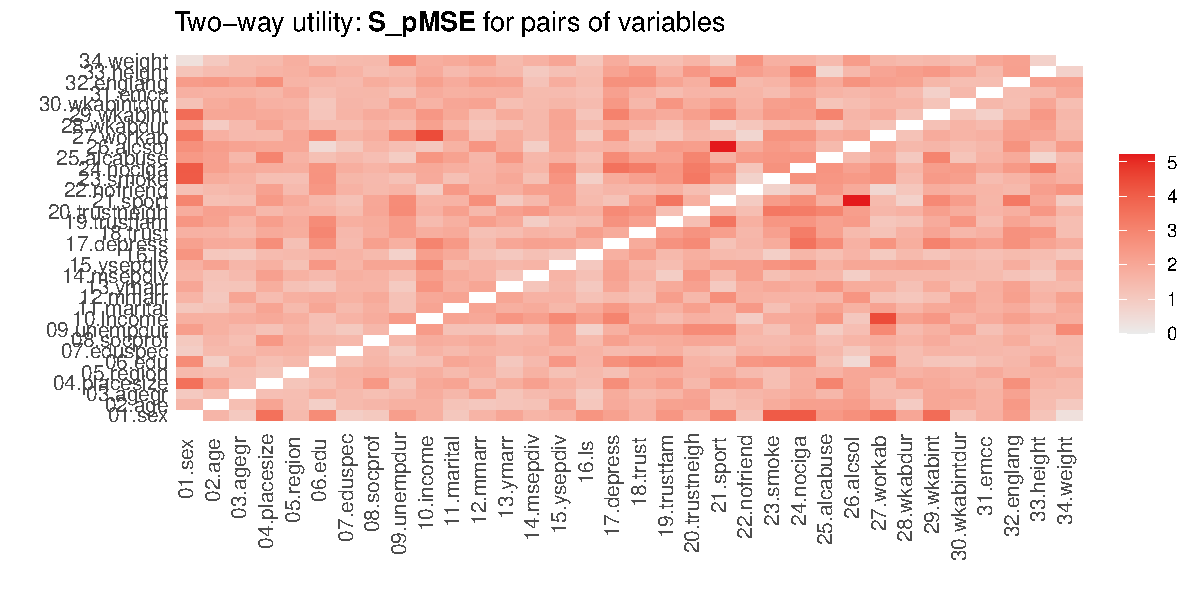
\includegraphics{../data/benchmark/graphs/synthpop/graph_synthpop_sd2011_bmi_two-way_utility.pdf}}
    \label{}
\end{figure}
}

\frame{\frametitle{DataSynthesizer utility - two-way utility}
\begin{figure}
    \caption{}
    \resizebox{\textwidth}{!}{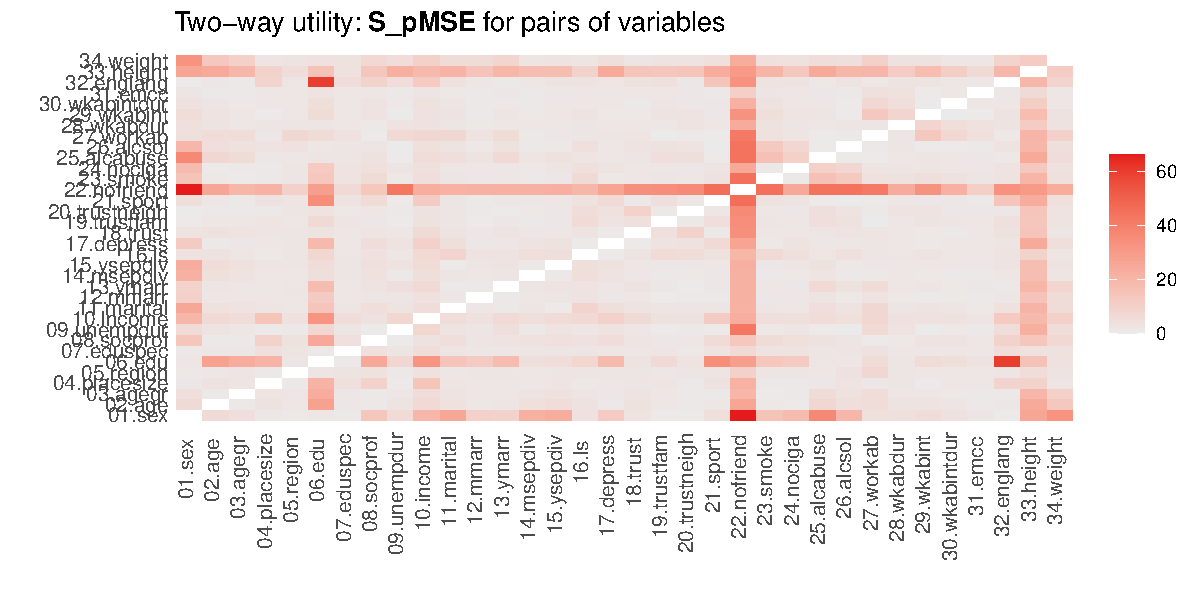
\includegraphics{../data/benchmark/graphs/datasynthesizer/graph_datasynthesizer_sd2011_bmi_two-way_utility.pdf}}
    \label{}
\end{figure}
}

\begin{frame}[fragile]{Kolmogorov-Smirnov statistic for full data set}

DataSynthesizer
\begin{lstlisting}[firstnumber=1, label=glabels, xleftmargin=10pt,frame=single] 
> utility_measure <- utility.gen(sds_list, df_ods, print.stats = "all", nperms = 3)
> utility_measure$SPECKS
     D 
0.5122 
\end{lstlisting}
Synthpop
\begin{lstlisting}[firstnumber=1, label=glabels, xleftmargin=10pt,frame=single] 
> utility_measure$SPECKS
     D 
0.2702 
\end{lstlisting}

\end{frame}

\begin{frame}[fragile]{Kolmogorov-Smirnov statistic for each variable}

DataSynthesizer
\begin{lstlisting}[firstnumber=1, label=glabels, xleftmargin=10pt,frame=single] 
> df_compare$tab.utility[,4]
       sex        age      agegr  placesize     region        edu    eduspec    socprof 
    0.0022     0.0220     0.0172     0.0040     0.0268     0.0088     0.0216     0.0160 
  unempdur     income    marital      mmarr      ymarr    msepdiv    ysepdiv         ls 
    0.0042     0.0376     0.0088     0.0088     0.0160     0.0038     0.0086     0.0060 
   depress      trust   trustfam trustneigh      sport   nofriend      smoke     nociga 
    0.0048     0.0026     0.0014     0.0042     0.0036     0.1566     0.0048     0.0076 
  alcabuse     alcsol     workab    wkabdur    wkabint wkabintdur       emcc    englang 
    0.0018     0.0010     0.0008     0.0040     0.0016     0.0020     0.0036     0.0072 
    height     weight 
    0.0948     0.0392
\end{lstlisting}
Synthpop
\begin{lstlisting}[firstnumber=1, label=glabels, xleftmargin=10pt,frame=single] 
> df_compare$tab.utility[,4]
       sex        age      agegr  placesize     region        edu    eduspec    socprof 
    0.0108     0.0164     0.0148     0.0122     0.0230     0.0096     0.0150     0.0172 
  unempdur     income    marital      mmarr      ymarr    msepdiv    ysepdiv         ls 
    0.0142     0.0198     0.0122     0.0112     0.0148     0.0044     0.0062     0.0020 
   depress      trust   trustfam trustneigh      sport   nofriend      smoke     nociga 
    0.0194     0.0046     0.0068     0.0102     0.0086     0.0036     0.0098     0.0146 
  alcabuse     alcsol     workab    wkabdur    wkabint wkabintdur       emcc    englang 
    0.0012     0.0010     0.0088     0.0018     0.0036     0.0050     0.0062     0.0122 
    height     weight 
    0.0110     0.0062 
\end{lstlisting}

\end{frame}


\frame{\frametitle{Synthpop utility - CIO}
\begin{figure}
    \caption{DV = log(income)}
    \resizebox{\textwidth}{!}{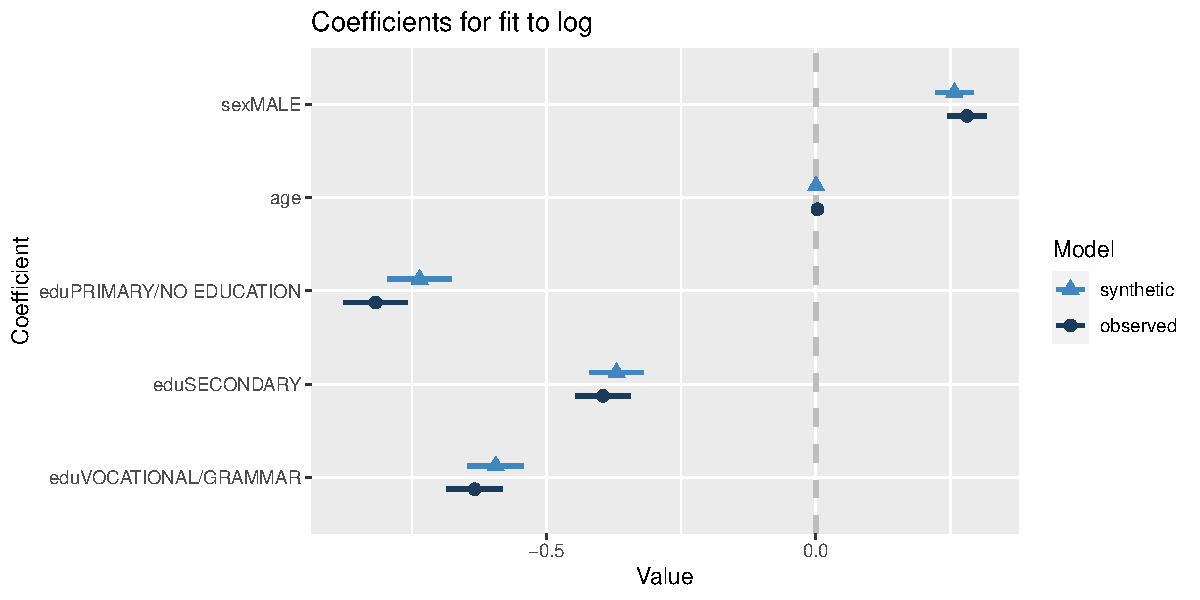
\includegraphics{../data/benchmark/graphs/synthpop/graph_synthpop_sd2011_bmi_cio.pdf}}
    \label{}
\end{figure}
}

\frame{\frametitle{DataSynthesizer utility - CIO}
\begin{figure}
    \caption{DV = log(income)}
    \resizebox{\textwidth}{!}{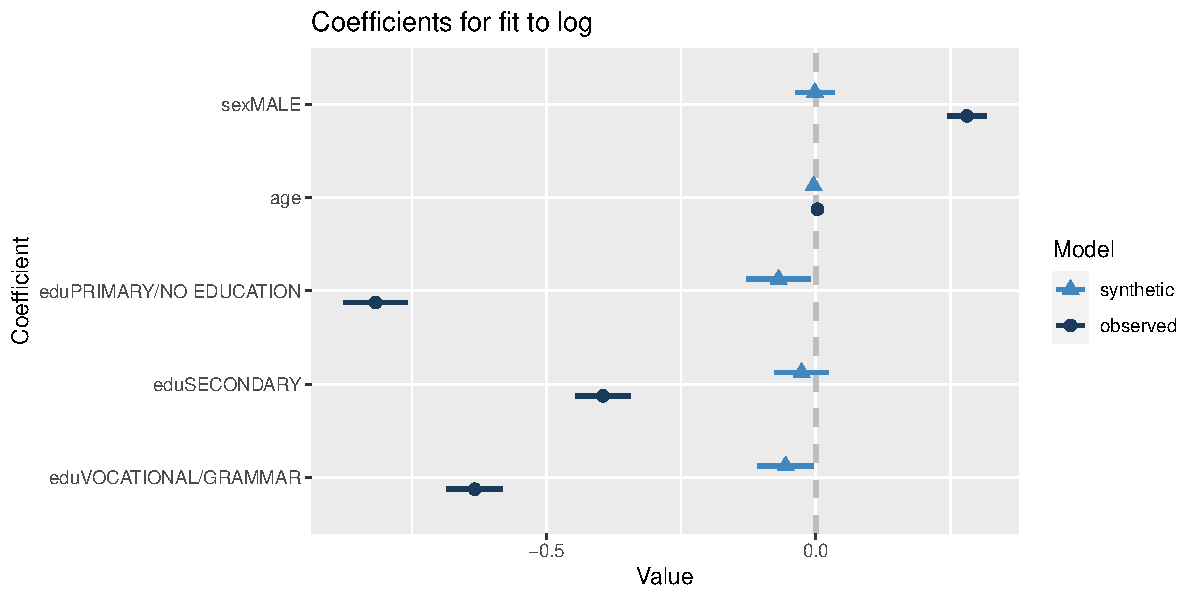
\includegraphics{../data/benchmark/graphs/datasynthesizer/graph_datasynthesizer_sd2011_bmi_cio.pdf}}
    \label{}
\end{figure}
}

\section{Conclusion}

\frame{\frametitle{}
\begin{itemize}
    \item Synthpop may not always be efficient
    \item How does Synthpop achieve such high levels of utility?
\end{itemize}

}


\end{document}


